\documentclass[11pt]{article}
\usepackage[a4paper,text={17cm,24cm},left=2cm,top=3cm]{geometry}
\usepackage[utf8]{inputenc}
\usepackage[IL2]{fontenc}
\usepackage[czech]{babel}
\usepackage{times}
\usepackage[unicode]{hyperref}
\usepackage{multirow}
\usepackage{multicol}
\usepackage{amsfonts}
\usepackage{amsmath}
\usepackage{amsthm}
\usepackage[ruled,vlined,linesnumbered,czech]{algorithm2e}
\usepackage{graphics}
\usepackage{pdflscape}
\usepackage{pict2e}
\usepackage{picture}
\usepackage{xurl}
\usepackage{float}


\begin{document}

     \begin{titlepage}
        \begin{center}
            \Huge
                \textsc{Vysoké učení technické v~Brně}
                
            \huge
                \textsc{Fakulta informačních technologií}
                
            \vspace{\stretch{0.3}}
            \LARGE
                Typografie a~publikování -- 3. projekt
                
            \Huge
                \textmd{Tabulky a~obrázky}
                
            \vspace{\stretch{0.4}}
        \end{center}
        {\Large 3. dubna 2021 \hfill Roman Popelka (xpopel24)}
    \end{titlepage}
\section{Úvodní strana}
Název práce umístěte do zlatého řezu a nezapomeňte uvést dnešní datum a vaše jméno a příjmení.
\section{Tabulky}
Pro sázenní tabulek můžeme použít buď prostředí\texttt{ tabbing } nebo prostředí\texttt{ tabular}.
\subsection{Prostředí\texttt{ tabbing}}
Pří použití\texttt{ tabbing }vypadá tabulka následnovně:
\begin{tabbing}
Vodní melouny\quad\=25,90\quad\=\textbf{Množství} \kill
\textbf{Ovoce} \> \textbf{Cena} \> \textbf{Množství} \\
Jablka         \>      25,90    \> 3 kg     \\
Hrušky         \>      27,40    \> 2,5 kg   \\
Vodní melouny  \>      35,--    \> 1 kus    \\
\end{tabbing}
Toto prostředí se dá také použít pro sázení algoritmů, ovšem vhodnější je použít prostředí\texttt{ algorithm }nebo \texttt{algorithm2e }(viz sekce \ref{sec3}).

\subsection{Prostředí\texttt{ tabular}}
Další možností, jak vytvořit tabulky, je použít prostředí\texttt{ tabular}. Tabulky pak budou vypadat takto\footnote{Kdyby byl problém s~\texttt{cline}, zkuste se podívat třeba sem: \url{ http://www.abclinuxu.cz/tex/poradna/show/325037}.\vfill}:

\vspace{5mm}
\begin{table}[ht]
    \begin{center} \catcode `\-=12
        \begin{tabular}{|c|c|c|}\hline
                          & \multicolumn{2}{c}{\textbf{Cena}}\vline \\ \cline{2-3}
            \textbf{Měna} & \textbf{nákup}  & \textbf{prodej} \\ \hline
              EUR         & 25,227          &     26,943      \\ 
              GBP         & 29,368          &     31,492      \\
              USD         & 21,260          &     22,661      \\ \hline
        \end{tabular}
        \caption{Tabulka kurzů k dnešnímu dni}
        \label{tab1}
    \end{center}
\end{table}

\begin{table}[ht]
    \catcode `\-=12
    \centering
    \begin{tabular}{|c|c|}\hline
         $A$        & $\neg A$   \\ \hline
         \textbf{P} & N          \\ \hline
         \textbf{O} & O          \\ \hline
         \textbf{X} & X          \\ \hline
         \textbf{N} & P          \\ \hline
    \end{tabular}
    \begin{tabular}{|c|c|c|c|c|c|}\hline
     \multicolumn{2}{|c|}{\multirow{2}{*}{$A \wedge B$}} & \multicolumn{4}{|c|}{B} \\ \cline{3-6}
     \multicolumn{2}{|c|}{}             & \textbf{P} & \textbf{O} & \textbf{X} & \textbf{N} \\ \hline
     \multirow{4}{*}{A}                 & \textbf{P} & P          &     O      & X          &  N \\\cline{2-6}
                                        & \textbf{O} & O          &     O      & N          &  N \\\cline{2-6}
                                        & \textbf{X} & X          &     N      & X          &  N \\\cline{2-6}
                                        & \textbf{N} & N          &     N      & N          &  N \\\hline
    \end{tabular}
     \begin{tabular}{|c|c|c|c|c|c|}\hline
     \multicolumn{2}{|c|}{\multirow{2}{*}{$A \vee B$}} & \multicolumn{4}{|c|}{B} \\ \cline{3-6}
     \multicolumn{2}{|c|}{}                                 & \textbf{P} & \textbf{O} & \textbf{X} & \textbf{N} \\ \hline
     \multirow{4}{*}{A}                 & \textbf{P} & P          &     P      & P          &  P \\\cline{2-6}
                                        & \textbf{O} & P          &     O      & P          &  O \\\cline{2-6}
                                        & \textbf{X} & P          &     P      & X          &  X \\\cline{2-6}
                                        & \textbf{N} & P          &     O      & X          &  N \\\hline
    \end{tabular}
    \begin{tabular}{|c|c|c|c|c|c|}\hline
     \multicolumn{2}{|c|}{\multirow{2}{*}{$A \rightarrow B$}} & \multicolumn{4}{|c|}{B} \\ \cline{3-6}
     \multicolumn{2}{|c|}{}             & \textbf{P} & \textbf{O} & \textbf{X} & \textbf{N} \\ \hline
     \multirow{4}{*}{A}                 & \textbf{P} & P          &     O      & X          &  N \\\cline{2-6}
                                        & \textbf{O} & P          &     O      & P          &  O \\\cline{2-6}
                                        & \textbf{X} & P         &     P      & X          &  X \\\cline{2-6}
                                        & \textbf{N} & P          &     P      & P          &  P \\\hline
    \end{tabular}
  
    \caption{Protože Kleeneho trojhodnotová logika je už \uv{zastaralá}, uvádíme si zde příklad čtyřhodnotové logiky}
    \label{tab2}
\end{table}
\pagebreak
\section{Algoritmy}\label{sec3}
Pokud budeme chtít vysázet algoritmus, můžeme použít prostředí\texttt{ algorithm\footnote{Pro nápovědu, jak zacházet s prostředím \texttt{ algorithm}, můžeme zkusit tuhle stránku:\\
\url{http://ftp.cstug.cz/pub/tex/CTAN/macros/latex/contrib/algorithms/algorithms.pdf}.} }  nebo \texttt{ algorithm2e}\footnote{Pro\texttt{ algorithm2e }zase tuhle:

\url{http://ftp.cstug.cz/pub/tex/CTAN/macros/latex/contrib/algorithm2e/doc/algorithm2e.pdf}.}. Příklad použití prostředí\texttt{ algorithm2e} viz Algoritmus \ref{alg1}.
\\\\
\begin{algorithm}[H]
\DontPrintSemicolon
\SetAlgoLongEnd
\SetNlSty{textmd}{}{:}
\SetKwInOut{Input}{Input}
\SetKwInOut{Output}{Output}
\KwIn{$(X_{t-1},u_t,z_t)$}
\KwOut{$X_t$}

\vspace{2mm}

\Indp\Indpp
\SetNlSkip{-1.2em}
$\overline{X_t} = X_t = 0$\;
\textbf{for} $k = 1 \text{ to } M$ \textbf{do}\;
\Indp\Indpp 
$x_{t}^{[k]} = sample\_motion\_model(u_t,x_{t-1}^{[k]})$\;
$w_{t}^{[k]} = measurement\_model(z_t,x_{t}^{[k]},m_{t-1})$\;
$m_{t}^{[k]} = updated\_occupancy\_grid(z_{t},x_{t}^{[k]},m_{t-1}^{[k]})$\;
$\overline{X_t} = \overline{X_t} + \langle x_{x}^{[m]},\omega_{t}^{[m]}\rangle$\;
\Indm\Indmm
\textbf{end for}\;
\textbf{for} $k = 1 \text{ to } M$ \textbf{do}\;
\Indp\Indpp
draw $i$ with probability $\approx \omega_{t}^{[i]}$\;
add $\langle x_{x}^{[k]},m_{t}^{[k]}\rangle \text{ to } X_{t}$\;
\Indm\Indmm
\textbf{end for}\;
\textbf{return} $X_t$
\caption{\textsc{\large{Fast}SLAM}}
\label{alg1}
\end{algorithm}
\vfill
\section{Obrázky}
Do našich článků můžeme samozřejmě vkládat obrázky. Pokud je obrázkém fotografie, můžeme klidně použít bitmapový soubor. Pokud by to ale mělo být nějaké schéma nebo něco podobného, je dobrým zvykem takovýto obrázek vytvořit vektorově.

\begin{figure}[h]
    \centering
    \scalebox{0.4}{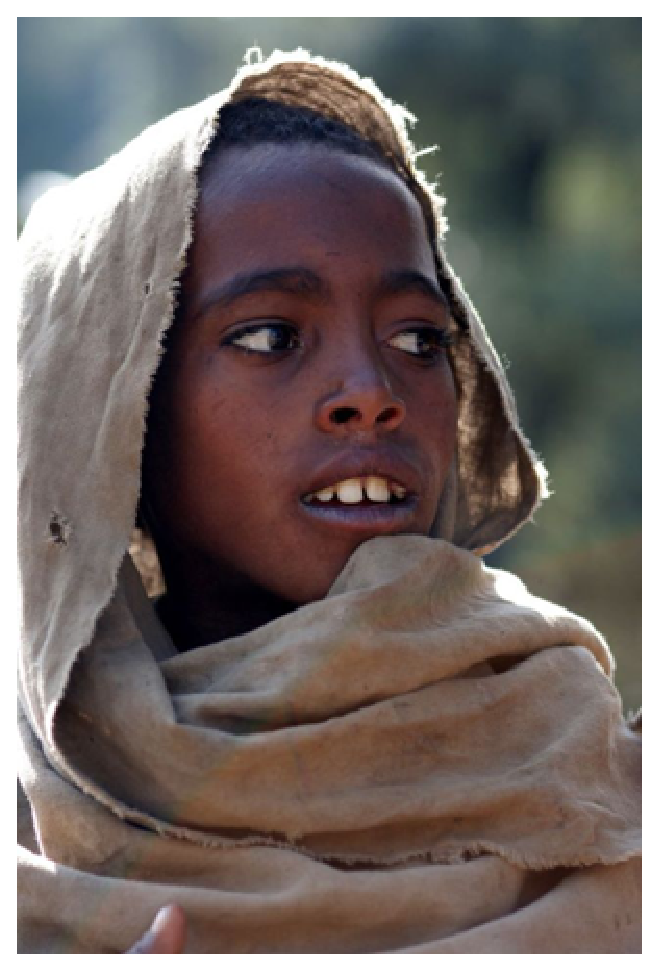
\includegraphics{etiopan.eps} 
    \reflectbox{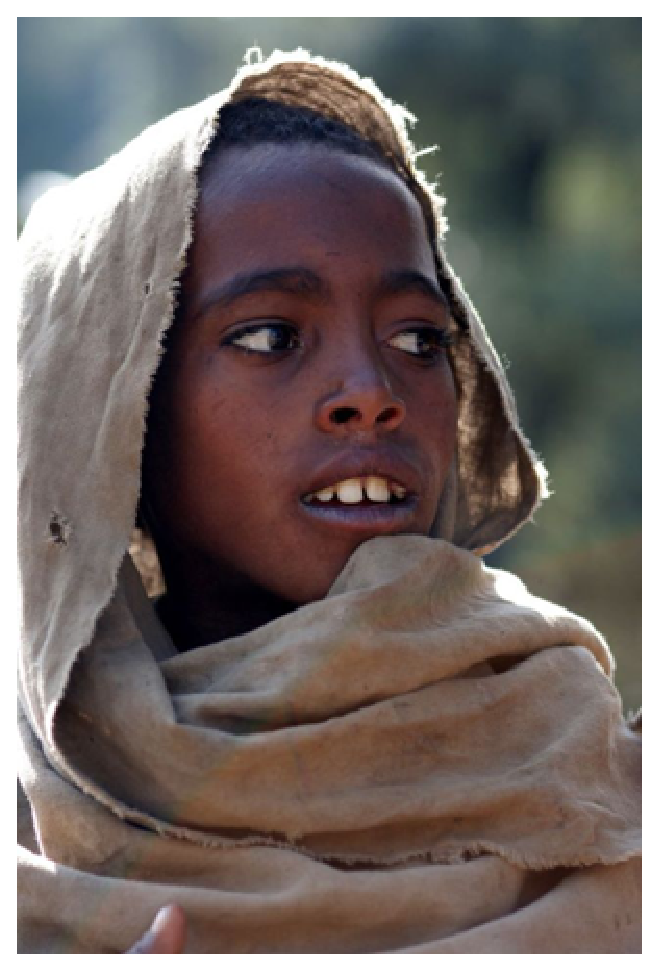
\includegraphics{etiopan.eps}}}
    \caption{Malý Etiopiánek a jeho bratříček}
    \label{obr1}
\end{figure}
\newpage

\quad Rozdíl mezi vektorovým$\ldots$

\begin{figure}[ht]
    \centering
    \scalebox{0.4}{
\includegraphics{oniisan.eps}}
    \caption{Vektorový obrázek}
    \label{obr2}
\end{figure}
$\ldots$ a bitmapovým obrázkem
\begin{figure}[ht]
    \centering
    \scalebox{0.57}{
\includegraphics{oniisan2.eps}}
    \caption{Bitmapový obrázek}
    \label{obr3}
\end{figure}

se projeví například při zvětšení.

\quad Odkazy (nejen ty) na obrázky \ref{obr1}, \ref{obr2} a~\ref{obr3}, na tabulky \ref{tab1} a~\ref{tab2} a~také na algoritmus \ref{alg1} jsou udělány pomocí~křížových 

odkazů. Pak je ovšem potřeba zdrojový soubor přeložit dvakrát.

\quad Vektorové obrázky lze vytvořit přímo v \LaTeX u, například pomocí prosředí\texttt{ picture}.
\pagebreak

\begin{landscape}
    \begin{figure}[ht]
        \centering
        \begin{picture}(320,320)
            \thicklines
            \put(40,0){\line(320,0){280}}
            \put(40,0){\line(0,40){40}}
            \put(40,0){\line(0,40){40}}
            \put(320,0){\line(0,1){40}}
            \put(40,40){\line(1,0){280}}
            \multiput(45, 40)(5, 0){56}{\line(0,1){20}}
            \multiput(45,60)(10,0){28}{\line(1,1){2.5}}
            \multiput(50,45)(10,0){27}{\line(1,0){5}}
            \multiput(50,47.5)(10,0){27}{\line(1,0){5}}
            \multiput(50,55)(10,0){27}{\line(1,0){5}}
            \multiput(50,57.5)(10,0){27}{\line(1,0){5}}
            \multiput(50,60)(10,0){28}{\line(-1,1){2.5}}
            
            \put(0,0){\line(0,1){110}}
            \put(5,0){\line(0,1){35}}
            \put(5,35){\line(-1,0){5}}
            \put(0,0){\line(1,0){5}}
            \put(5,0){\line(1,0){35}}
            \put(5,10){\line(1,0){35}}
            \put(5,20){\line(1,0){35}}
            \put(5,30){\line(1,0){35}}
            \put(5,40){\line(1,0){35}}
            \put(5,35){\line(0,1){75}}
            \put(0,110){\line(1,0){5}}
            \put(40,35){\line(0,1){75}}
            \put(0,110){\line(1,0){320}}
            \put(320,40){\line(0,1){70}}
            \put(0,110){\line(0,1){100}}
            \put(320,110){\line(0,1){100}}
            \put(0,210){\line(1,0){320}}
            \put(60,130){\line(1,0){60}}
            \put(60,130){\line(0,1){30}}
            \put(60,160){\line(1,0){60}}
            \put(120,160){\line(0,-1){30}}
            \put(230,130){\line(1,0){60}}
            \put(230,130){\line(0,1){30}}
            \put(230,160){\line(1,0){60}}
            \put(290,160){\line(0,-1){30}}
            \put(5,110){\line(0,1){50}}
            \put(40,110){\line(0,1){50}}
            \put(5,160){\line(1,0){35}}
            \put(10,130){\circle{4}}
            \put(0,210){\line(4,3){160}}
            \put(320,210){\line(-4,3){160}}
            \put(320,300){\circle{60}}
            
        \end{picture}
        \caption{Moje obydlí}
        \label{obr4}
    \end{figure}
\end{landscape}

\end{document}
